\section{Performance} \label{sec:lhc:performance}

Since the begining of its stable running in 2010 the LHC has performed well,
exceeding expectations.  While the LHC operation itself is incredibly complex,
the performance of the machine, for the purposes of analysis, can be reduced to
three numbers; the familiar center of mass energy of the beams, the integrated
luminosity and the instantaneous luminosity.  

For particle physics the integrated luminosity is proportional to the total
number of collisions recorded during a specified time period, while the
instantaneous luminosity is a function of the number of protons per bunch, the
bunch crossing rate and the cross section of a proton-proton interaction and
represents the particle flux.  Knowing this one can see that the integrated
luminosity, $L_{int}$ is simply the integral of the instantaneous luminosity
$L_{\text{inst.}}$ for a chosen data period as seen in
\Cref{eq:integrated_luminosity}.

\begin{equation} \label{eq:integrated_luminosity}
   L_{\text{int}} = \int L_{\text{inst.}}dt 
\end{equation}

For a standard Gaussian beam, $L_{\text{inst.}}$ can be written as

\begin{equation} \label{eq:inst_luminosity}
  L_{\text{inst.}} = \frac{N_{b}^{2}n_{b}f_{\text{rev}}\gamma_{r}}{4\pi\epsilon_{n}\beta^{*}}F
\end{equation}

where $N_{b}$ is the number of particles per bunch, $n_{b}$ the number of
bunches per beam, $f_{\text{rev}}$ the revolution frequency, $\gamma_{r}$ the
relativistic gamma factor, $\epsilon_{n}$ the normalized transverse beam
emittance, $\beta^{*}$ the beta function at the collision point, and $F$ the
geometric luminosity reduction factor due to the crossing angle at the
interaction point given by

\begin{equation}
  F = \bigg(1 + \Big( \frac{\theta_{c}\sigma_{z}}{2\sigma^{*}} \Big) ^{2}
\bigg)^{-1/2} 
\end{equation}

where $\theta_{c}$ is the full crossing angle at the interaction point,
$\sigma_{z}$ is the RMS bunch length, and $\sigma^{*}$ is the transverse RMS
beam size at the interaction point \cite{Evans:2008zzb}. Nominal values for the
above quantities are shown in \Cref{table:nominal_values} which also
demonstrates the incredible success of the LHC operators and accelerator teams
during the LHC Run II data taking period.

\begin{table}[htpb]
 \centering
 \caption{
  Nominal design values of LHC operations parameters at ATLAS for $25~\textrm{ns}$ bunch crossing spacing~\cite{Evans:2008zzb,PhysRevAccelBeams.19.101003}.
  Design and ATLAS recorded values of the machine luminosity are also given for LHC Run II operations~\cite{TWiki:2018ATLASPeakLumi}.
 }
 \begin{tabular}{@{}llr@{}} \toprule
  Parameter                                   & Symbol             & LHC Run II Value                \\ \midrule
  LHC circumference                           &                    & $26,659~\mathrm{m}$             \\
  LHC design beam energy                      &                    & $7~\TeV$                        \\
  LHC beam energy in Run II                   &                    & $6.5~\TeV$                      \\
  Number of protons per bunch                 & $N_{b}$            & $1.15 \times 10^{11}$           \\
  Number of proton bunches per beam           & $n_{b}$            & $2,808$                         \\
  Revolution frequency                        & $f_{\textrm{rev}}$ & $11.245~\mathrm{kHz}$           \\
  Lorentz factor (design)                     & $\gamma_{r}$       & $7462.69$                       \\
  Lorentz factor at $\sqrt{s} = 13~\TeV$      &                    & $6929.64$                       \\
  Normalized transverse beam emittance        & $\epsilon_{n}$     & $3.75~\mu\mathrm{m}$            \\
  Collision point beta function               & $\beta^{*}$        & $0.55~\mathrm{m}$               \\
  Full crossing angle                         & $\theta_{c}$       & $285~\mu\mathrm{rad}$           \\
  RMS bunch length                            & $\sigma_{z}$       & $7.55\times 10^{-2}~\mathrm{m}$ \\
  Transverse RMS beam size                    & $\sigma^{*}$       & $16.6~\mu\mathrm{m}$            \\ \midrule
  Peak design machine luminosity at $13~\TeV$ & $L_{\text{inst.}}$ & $9~\inb\mathrm{s}^{-1}$         \\
  Peak ATLAS recorded machine luminosity      &                    & $21~\inb\mathrm{s}^{-1}$        \\
  \bottomrule
 \end{tabular}\label{table:nominal_values}
\end{table}

The ATLAS experiment integrated luminosity for each year can be seen in
\Cref{fig:intlumivsyear} along with an example of the instantaneous luminosity
for $2017$ in \Cref{fig:peakLumiByFill} which is used in the presented analysis.

\begin{figure}[!htbp] 
\centering
\subcaptionbox{Integrated Luminosity 2011 - 2018\label{fig:intlumivsyear}}{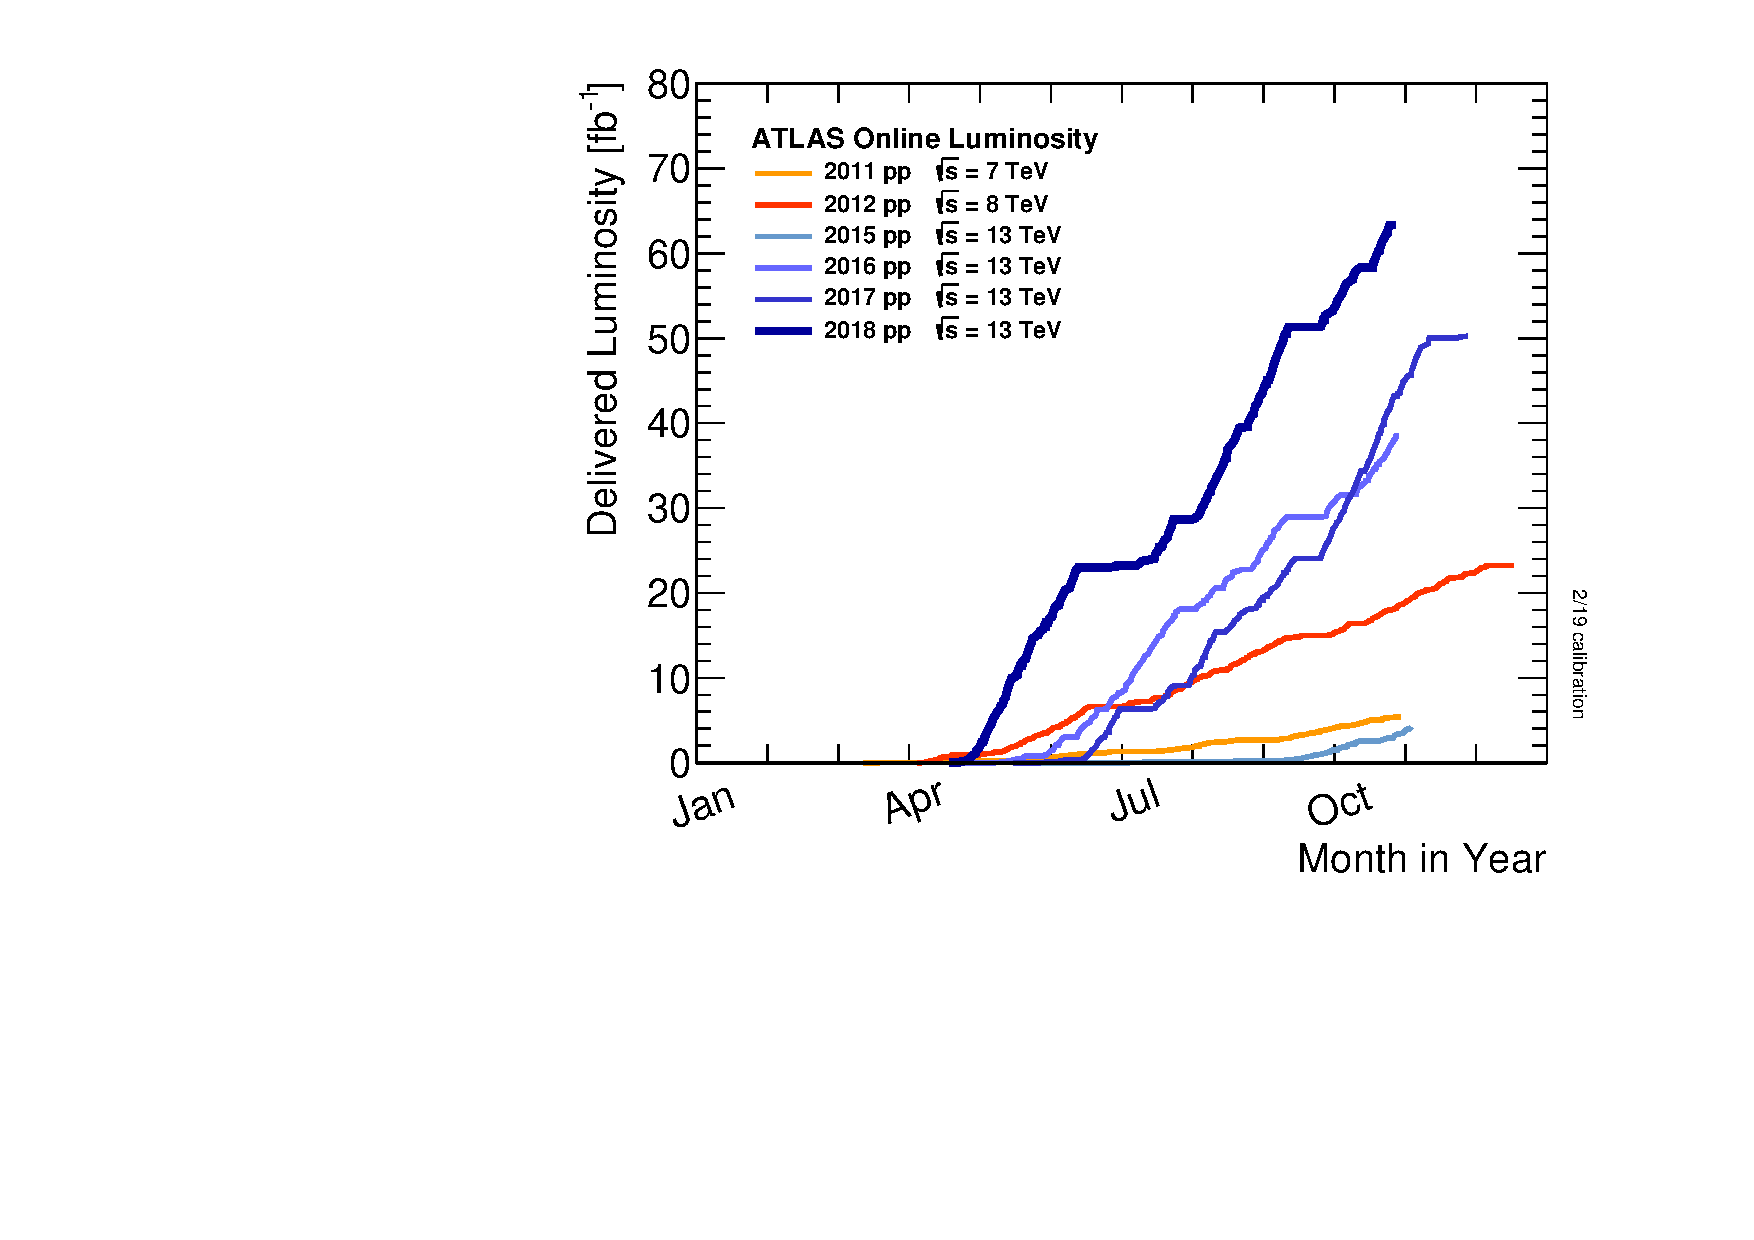
\includegraphics[width=0.5\textwidth]{figures/lhc/intlumivsyear.pdf}}\hfill
\subcaptionbox{2017 Peak Instantaneous Luminosity\label{fig:peakLumiByFill}}{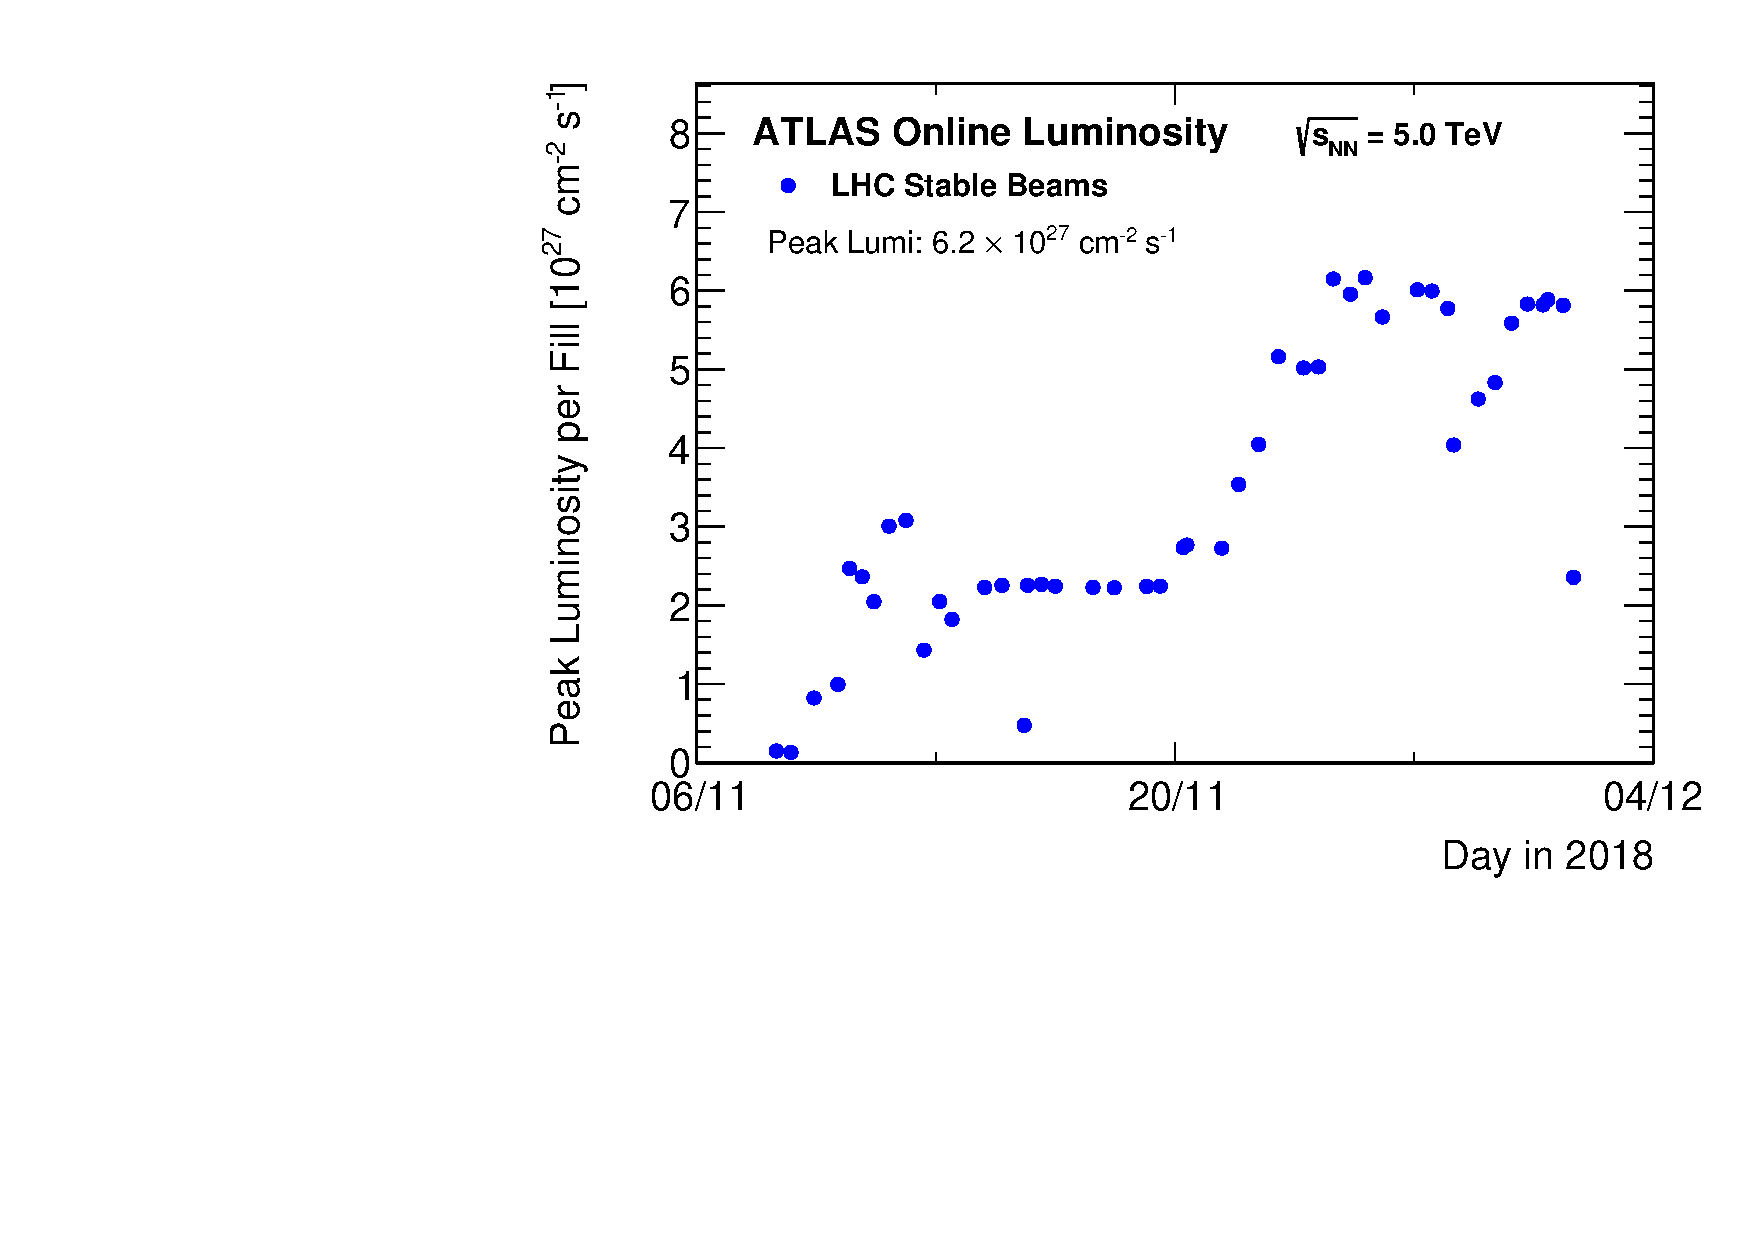
\includegraphics[width=0.5\textwidth]{figures/lhc/peakLumiByFill.pdf}}\hfill
\caption{Luminosity is monitored as both a running total known as the
Integrated Luminosity as depicted in (a) and as an instantaneous quantity as
shown in (b) \cite{LuminosityPublicResultsRun2}.}
\label{fig:luminosity} 
\end{figure}

